% Slides for 2024-05-31
% To create a slide, use the following:
% \begin{frame}{TITLE}
%     BODY
% \end{frame}

% To create a slide with a bullet list, use the following:
% \begin{frame}{TITLE}
%     \begin{itemize}
%         \item ITEM 1
%         \item ITEM 2
%     \end{itemize}    
% \end{frame}

% To create a slide with numbered list, use the following:
% \begin{frame}{TITLE}
%     \begin{enumerate}
%         \item ITEM 1
%         \item ITEM 2
%     \end{enumerate}
% \end{frame}

% To create a slide with a graphic:
% 1. Add the graphic to this folder (named picture.png)
% 2. Use the following:
% \begin{frame}{TITLE}
%     \centering
%     \includegraphics[height=0.7\textheight,width=0.7\textwidth,keepaspectratio]{picture.png}
% \end{frame}

% To create a slide with two columns, use the following:
% \begin{frame}{TITLE}
%     \begin{columns}
%         \begin{column}{0.5\textwidth}
%             COLUMN 1 BODY
%         \end{column}
%         \begin{column}{0.5\textwidth}
%             COLUMN 2 BODY
%         \end{column}
%     \end{columns}
% \end{frame}


\begin{frame}{Selecting Clips}
    \centering
    
\includegraphics[height=0.7\textheight,width=0.7\textwidth,keepaspectratio]{./images/clip_selection_process.png}
\end{frame}

\begin{frame}{Confidences}
    \begin{columns}
        \begin{column}{0.5\textwidth}
            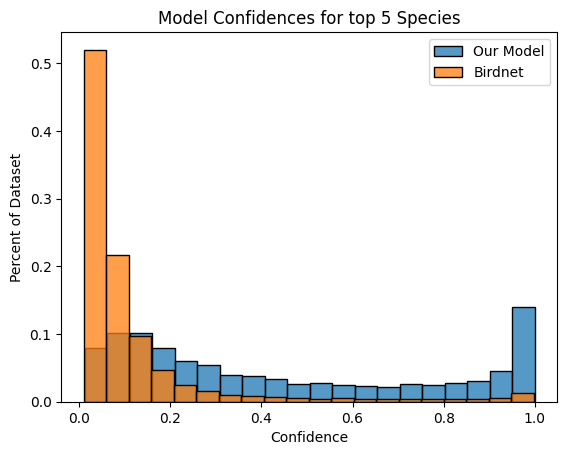
\includegraphics[height=0.7\textheight,width=0.7\textwidth,keepaspectratio]{./images/conf.png}
        \end{column}
        \begin{column}{0.5\textwidth}
            \begin{itemize}
                \item Birdnet is not Confidence
                \item Ours: 64 species >90\% confidence
                \item Birdnet: 16 species >90\% confidence
                \item We verified species were there
                \item Birdnet drops many "easy" examples
            \end{itemize}
        \end{column}
    \end{columns}
\end{frame}

\begin{frame}{Compare ROC}
    \begin{columns}
        \begin{column}{0.5\textwidth}
            \begin{itemize}
                \item Is this fair?
                \item Verified Clips based on Model Confidence
                \item Therefore clips verified differ
                \item test data: AM1 or the verified clips
            \end{itemize}
        \end{column}
        \begin{column}{0.5\textwidth}
            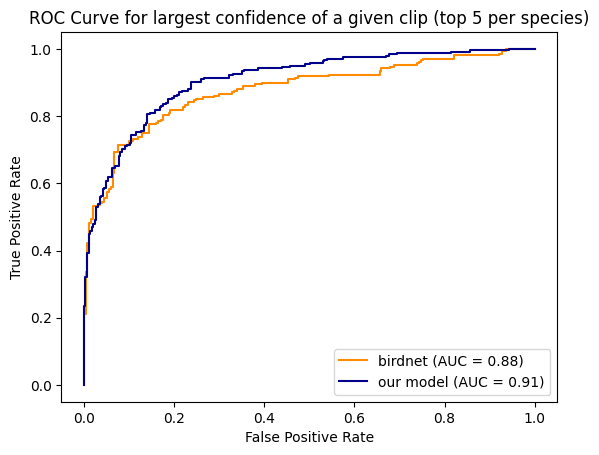
\includegraphics[height=0.7\textheight,width=0.7\textwidth,keepaspectratio]{./images/roc.png}
        \end{column}
    \end{columns}
\end{frame}

\begin{frame}{EGCI For 1000 Samples of Peru XC and Collaborator's Data}
    \centering
    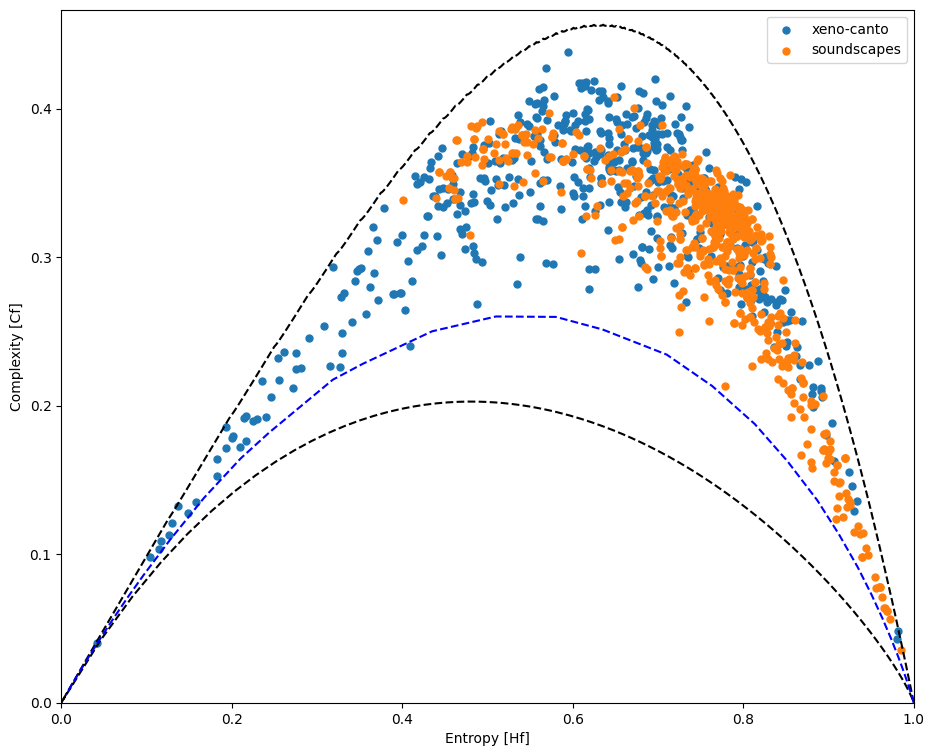
\includegraphics[height=0.7\textheight,width=0.7\textwidth,keepaspectratio]{./images/EGCI.png}
\end{frame}


\begin{frame}{CSE 145 Updates: Birdclef submissions}
    \centering
    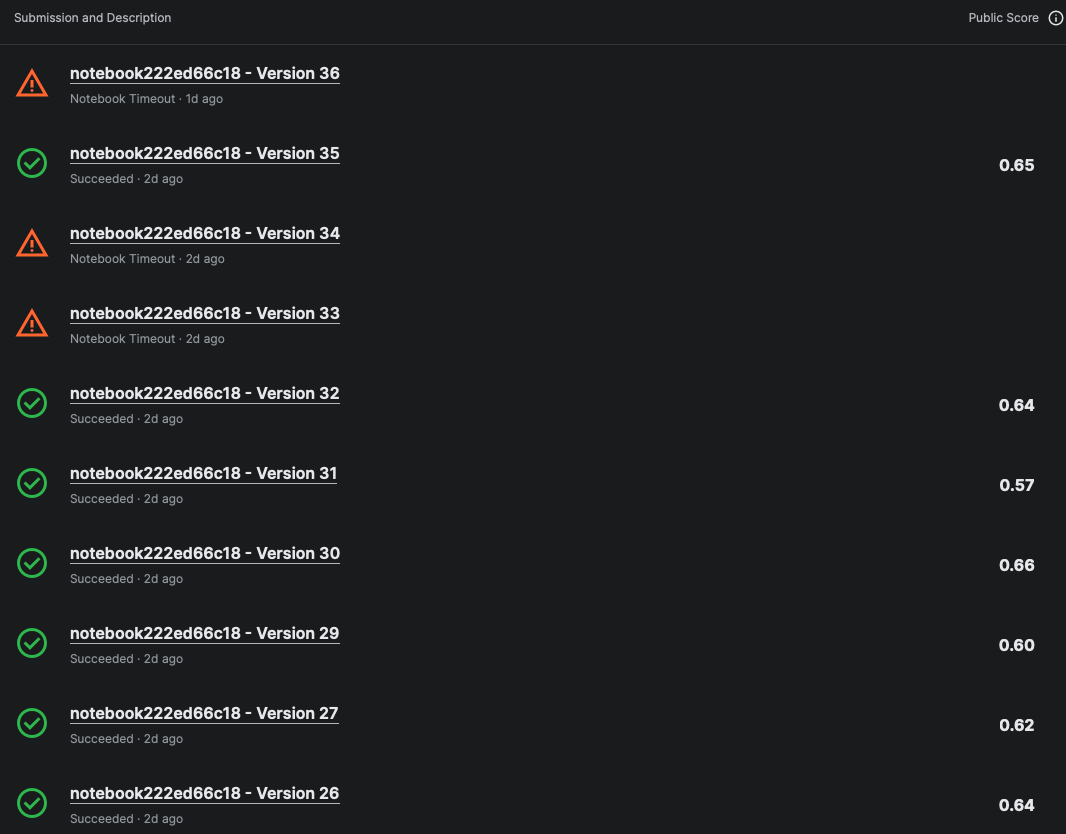
\includegraphics[height=0.7\textheight,width=0.7\textwidth,keepaspectratio]{images/Birdclef_submissions.png}
\end{frame}

% To create a slide with numbered list, use the following:
\begin{frame}{CSE 145 Updates}
    \begin{enumerate}
        \item Model submissions via Kaggle are working
        \item Currently working on Rust implementation
        \item Running ensemble after Rust implementation
        \item Mamba model finished training - evaluation
        \item Working on the final report
    \end{enumerate}
\end{frame}

\begin{frame}{Initial Template matching Results}
    \centering
    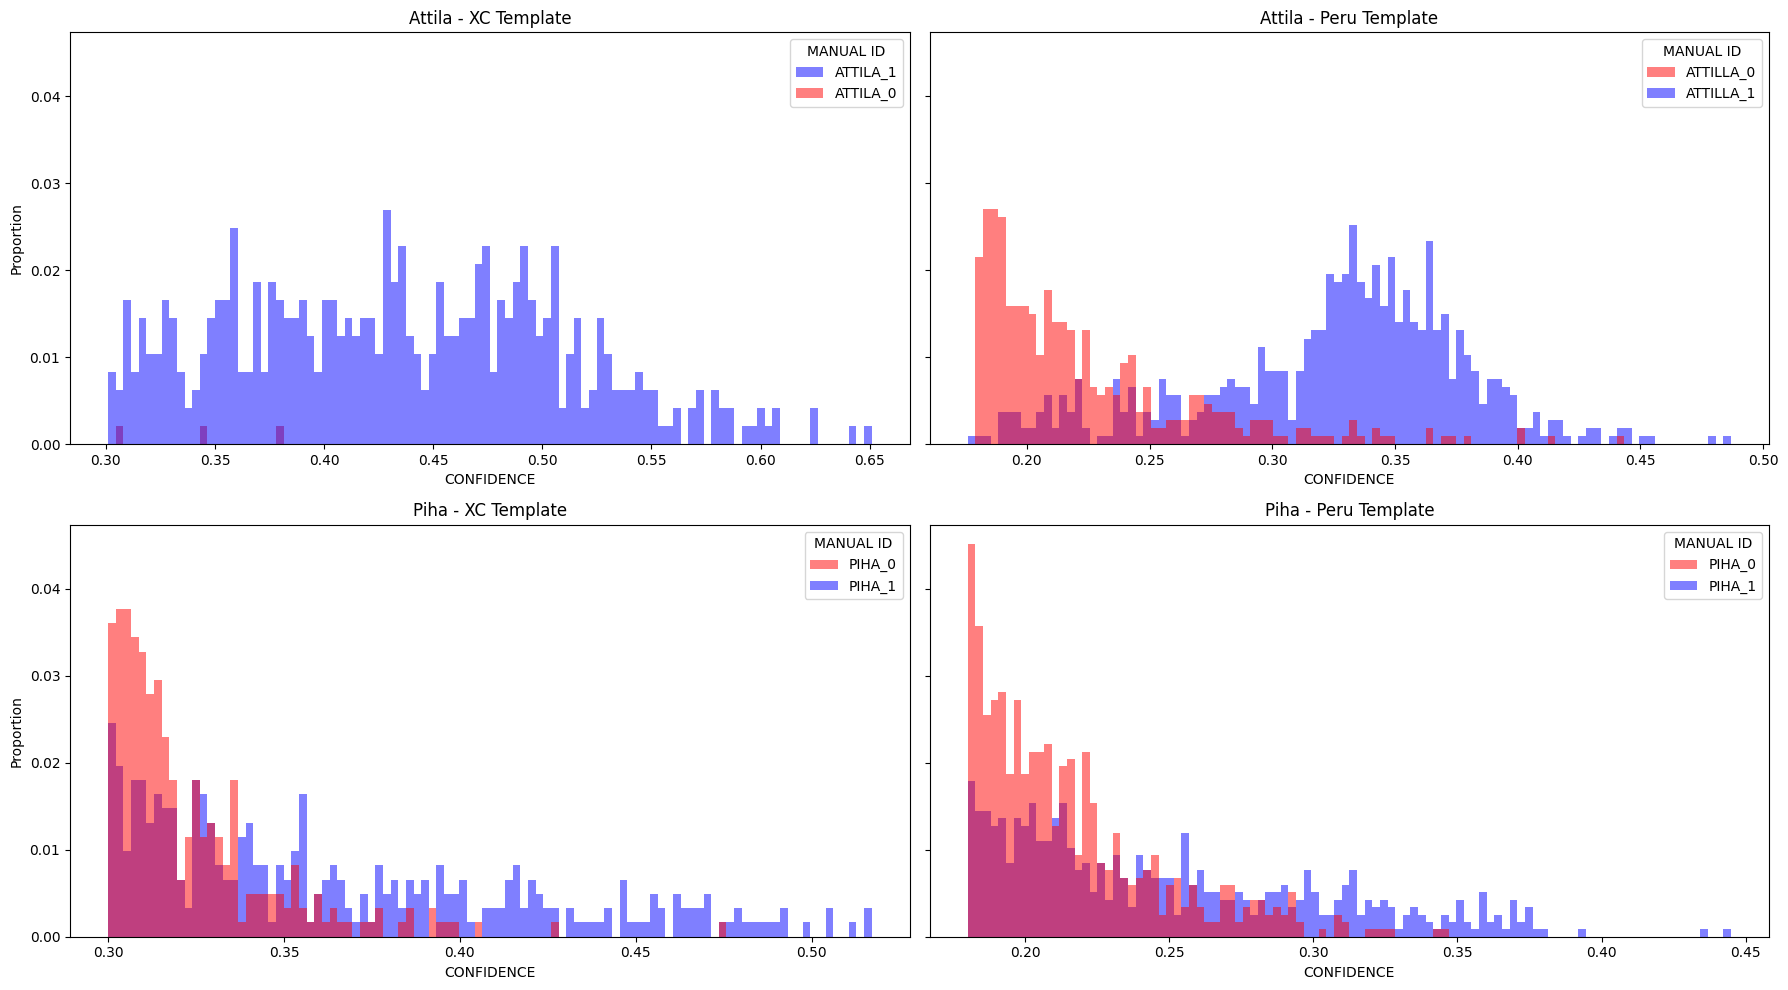
\includegraphics[height=0.9\textheight,width=0.9\textwidth,keepaspectratio]{images/conf_dists.png}

    Caveat: Different thresholds
\end{frame}

\begin{frame}{Efficientnet Performance}
    \centering
    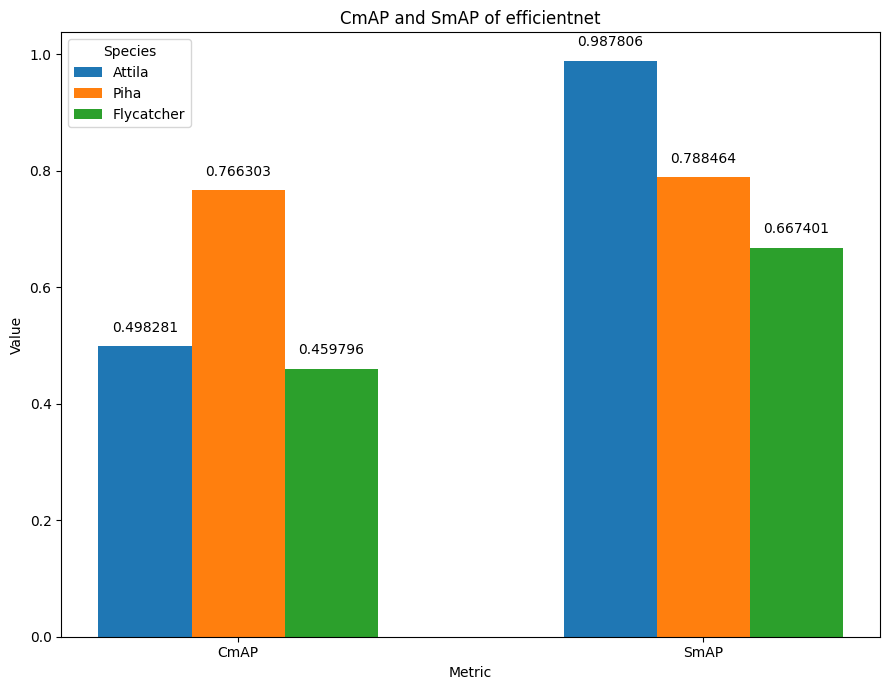
\includegraphics[height=0.7\textheight,width=0.7\textwidth,keepaspectratio]{images/cmap_smap_3species.png}

    CmAP: Class mean average precision

    SmAP: Sample mean average precision
\end{frame}

%HEY TQ I"M TALKING TO YOU PLEASE ADD ANY SMALL UPDATES HERE
\begin{frame}{Extra Discussions}
    \begin{itemize}
        \item The phones record in Stereo!
        \item Will start beamforming experiments
        \item JACOB'S THESIS DEFENSE 8AM MONDAY!!!!
    \end{itemize}
\end{frame}
%HEY TQ I"M TALKING TO YOU PLEASE ADD ANY SMALL UPDATES HERE



%MAKE SURE THAT IS THE LAST SLIDE TOO